\subsection{Cross-Language Acoustic Motivation for Emergency Sensitivity}
Our objective in this subsection is to motivate emergency-versus-normal separability, not to claim a cross-language SOTA result. We use a small five-language evidence pool (Chinese, English, French, Italian, and Polish) as design guidance. The evidence pipeline is documented in \texttt{analysis/cross\_language\_emergency/longrun\_multilingual\_commonality\_2026w14/final\_report\_en\_2026w14.md}, with registry and mapping details in \texttt{dataset\_registry\_2026w14.csv} and \texttt{mapping\_contract\_2026w14.md}. The mapping contract is fixed as: \emph{emergency = anger + fear}, \emph{normal = neutral (+ calm)}, and \emph{surprise} is used only for sensitivity analysis. We report feature effects using Cohen's $d$~\cite{cohen1988statistical} and track cross-language heterogeneity with $I^2$~\cite{higgins2003measuring}, while using public emotional speech resources as external anchors (ESD~\cite{zhou2021esd} and CREMA-D~\cite{cao2014cremad}).

\begin{figure}[t]
  \centering
  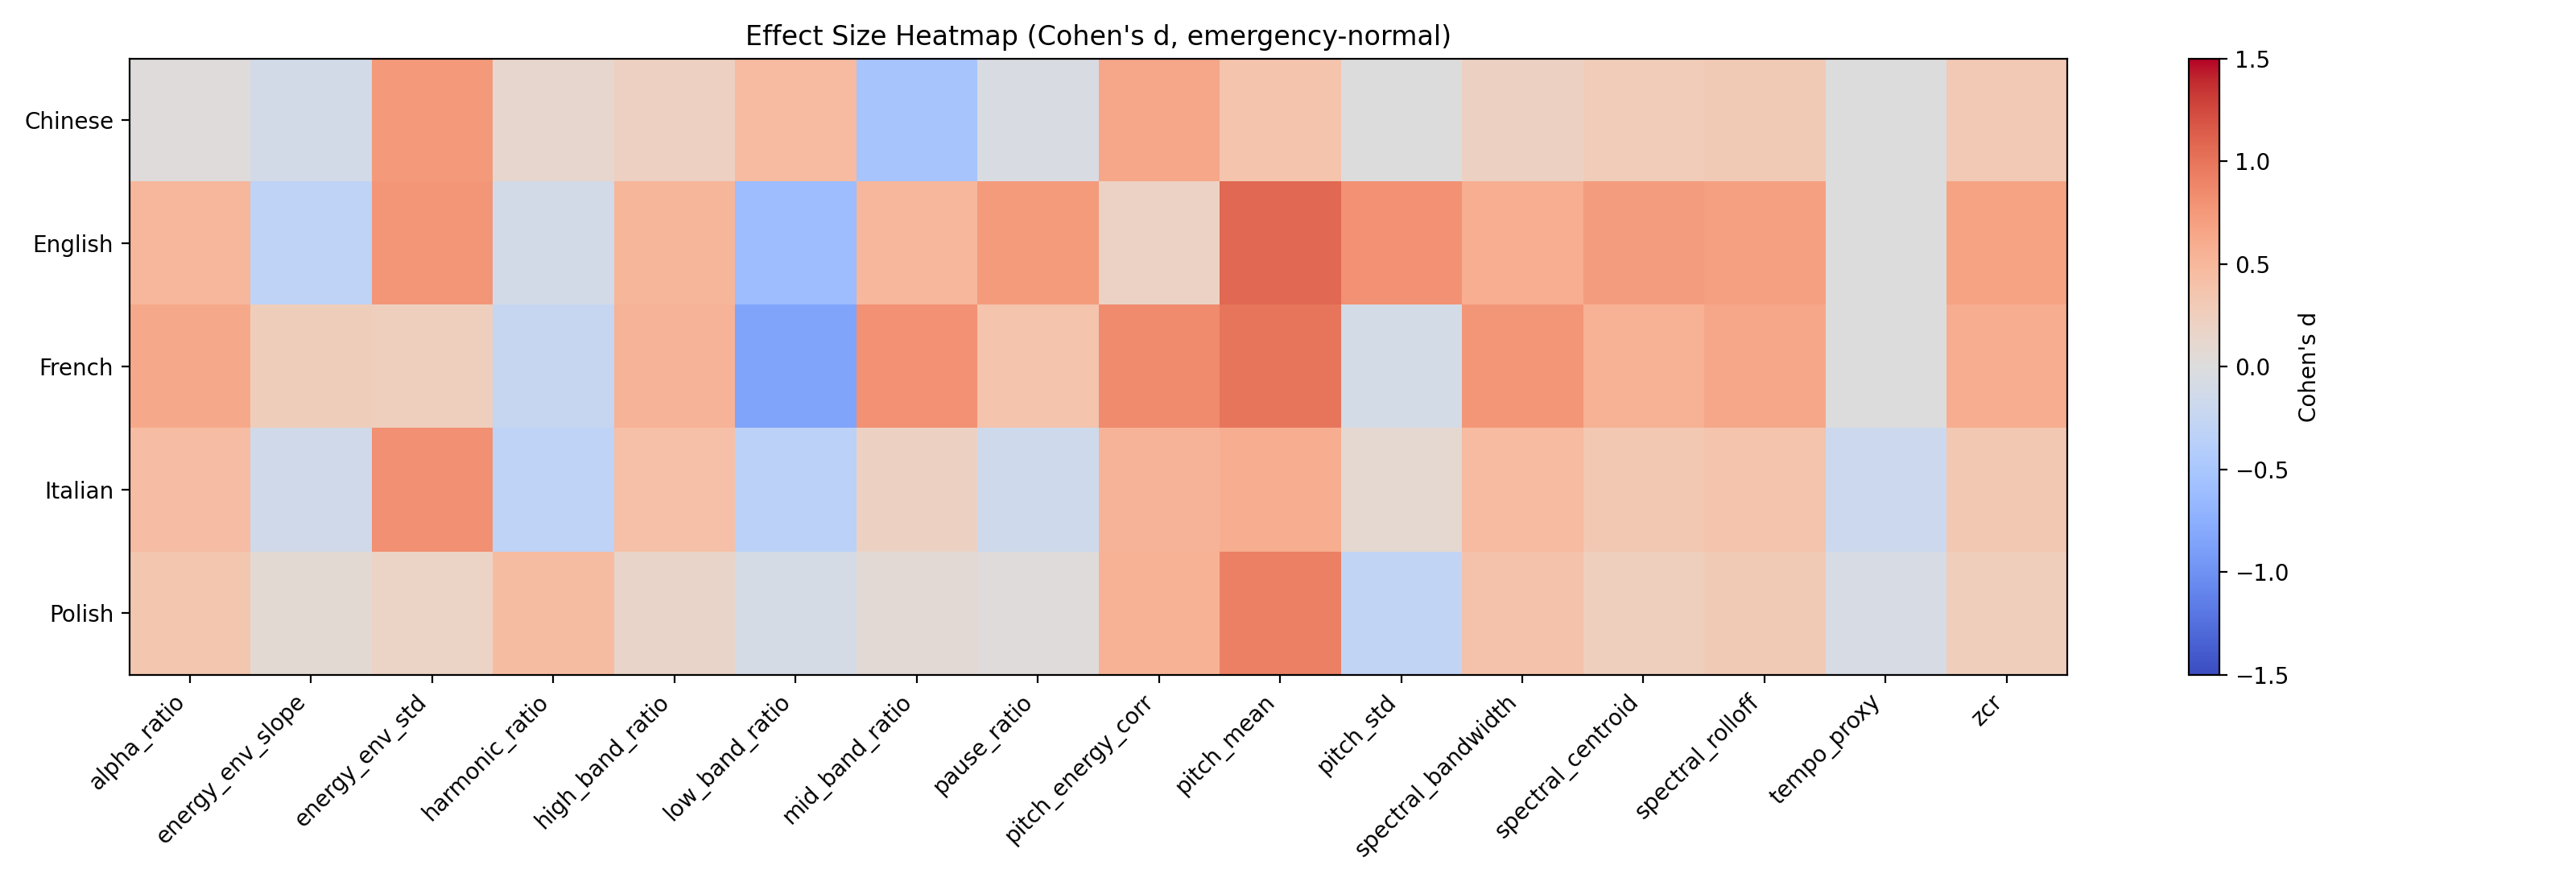
\includegraphics[width=\linewidth]{analysis/cross_language_emergency/longrun_multilingual_commonality_2026w14/figures/fig02_effectsize_heatmap_language_feature.png}
  \caption{Per-language emergency-vs-normal effect-size heatmap used for motivation analysis (five-language small-scale evidence; not a cross-language SOTA benchmark).}
  \label{fig:motivation_effectsize_heatmap}
\end{figure}

\begin{figure}[t]
  \centering
  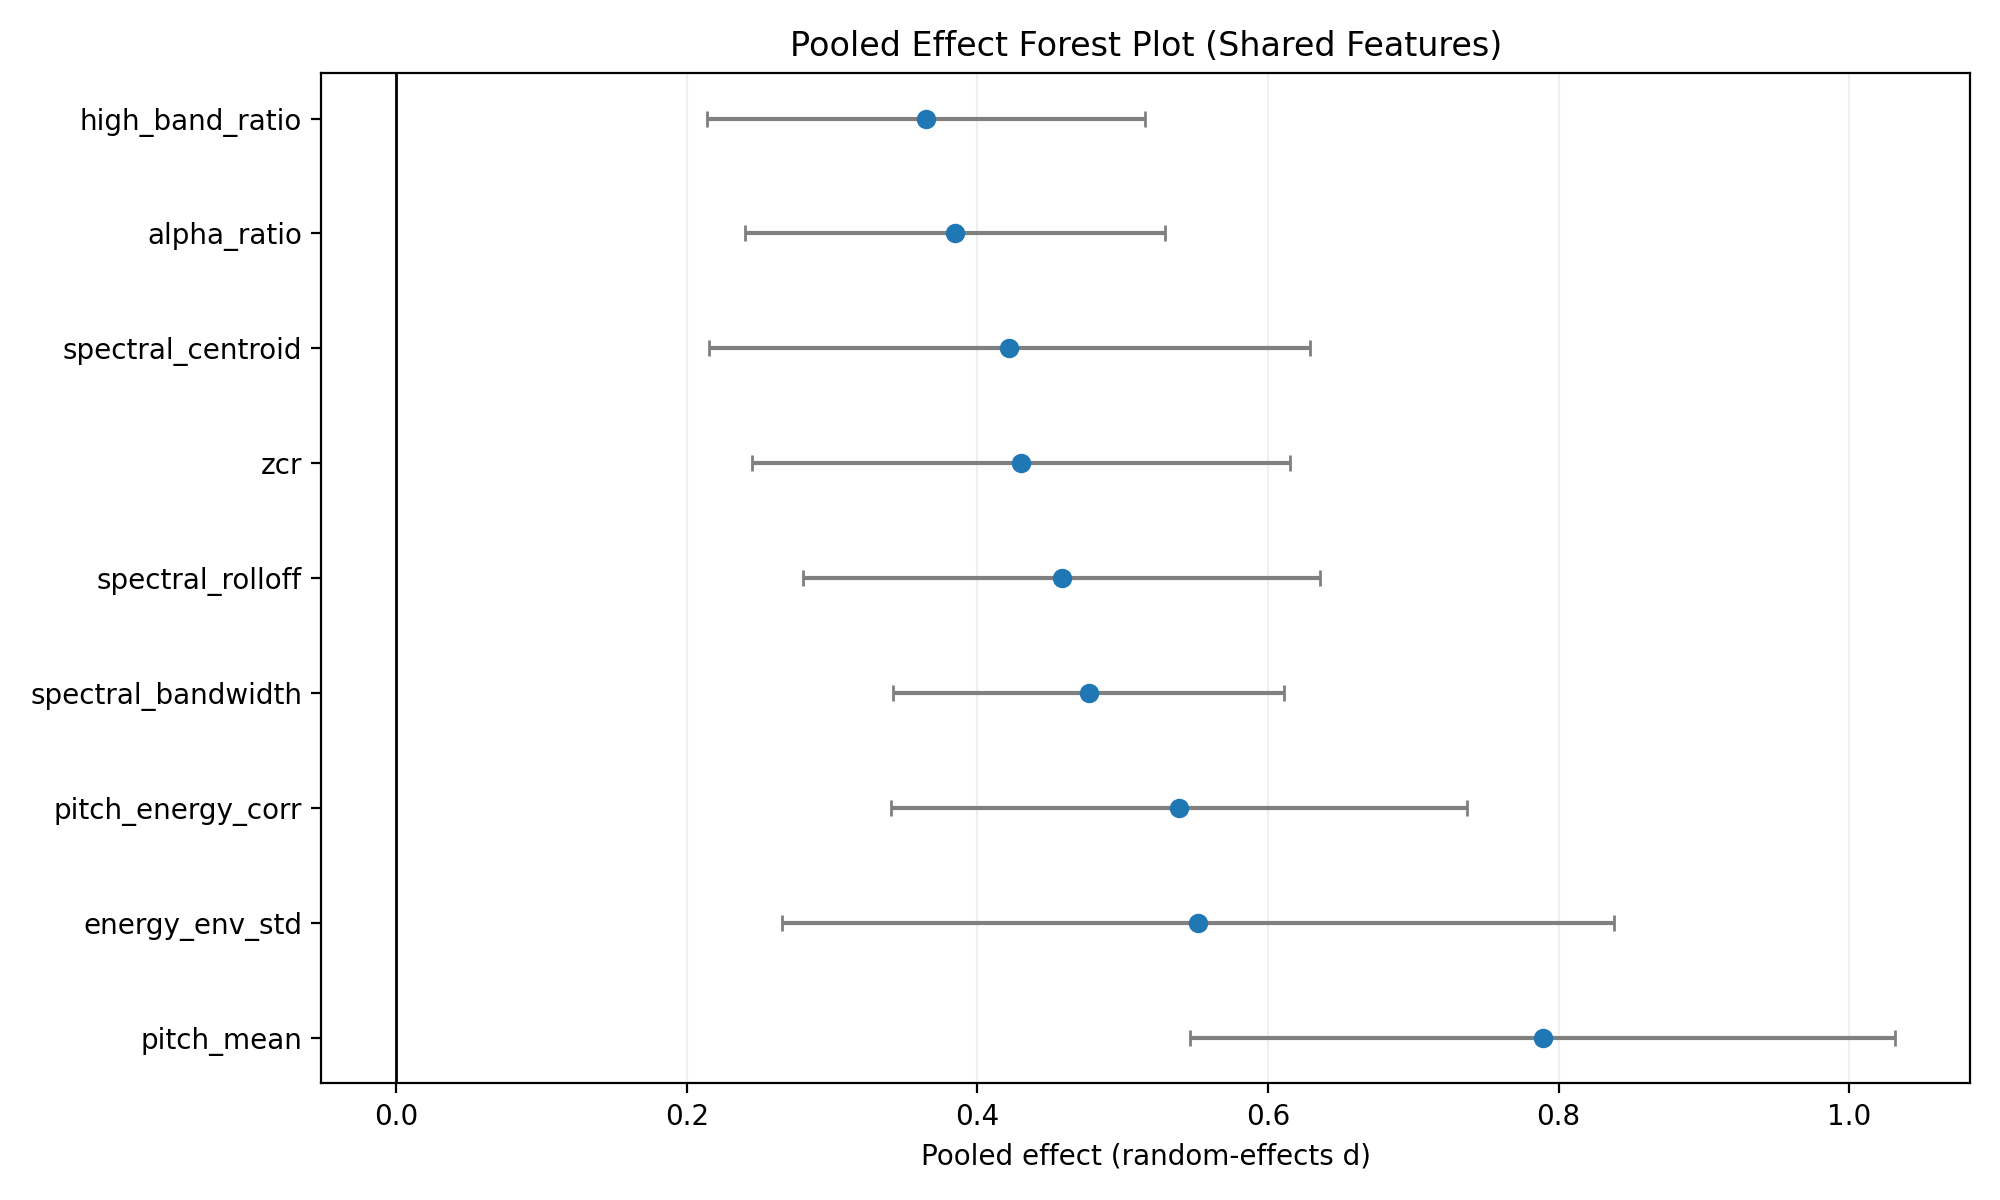
\includegraphics[width=\linewidth]{analysis/cross_language_emergency/longrun_multilingual_commonality_2026w14/figures/fig03_pooled_effect_forest_shared_features.png}
  \caption{Pooled effect forest for shared features used to derive training priors.}
  \label{fig:motivation_pooled_forest}
\end{figure}

Across the pooled analysis, \textbf{shared features: 9}. The top three shared features are:
\begin{itemize}
\item \textbf{pitch\_mean}: pooled $d=0.789$, $95\%$CI$=[0.546, 1.032]$
\item \textbf{energy\_env\_std}: pooled $d=0.552$, $95\%$CI$=[0.265, 0.838]$
\item \textbf{pitch\_energy\_corr}: pooled $d=0.539$, $95\%$CI$=[0.340, 0.737]$
\end{itemize}
These values support emergency sensitivity as an acoustic motivation signal and suggest that pitch-energy interaction cues should be preserved during training.

We explicitly keep two risks in scope. First, heterogeneity is non-negligible: $I^2$ is elevated for several pooled features, so cross-language consistency is partial rather than universal. Second, normal-class coverage is limited for some languages, which can bias pooled estimates. Therefore, in this paper, cross-language evidence is used to motivate design choices, not to prove multilingual generalization gains.
